\chapter{Теоретическая часть}

\section{Развитие генераторов сигналов}
История развития генераторов сигналов начинается с аналоговых устройств, которые
использовались для генерации различных форм сигналов, включая низкочастотные,
высокочастотные, сверхвысокочастотные и импульсные. <<Во времена СССР потребности в новых средствах генерации сигналов удовлетворялись разработкой огромного числа всевозможных аналоговых генераторов сигналов>>~\cite{dgs}. Однако, с развитием технологий и потребностями в более сложных и модулируемых сигналах, стало очевидно необходимость в универсальных генераторах сигналов, способных генерировать сигналы типовых форм, такие как синусоидальные, прямоугольные, пилообразные и треугольные.

В результате развития технологий и потребностей в более сложных и модулируемых
сигналах, появились новейшие разработки генераторов сигналов на основе прямого
цифрового синтеза частот и форм сигналов. Эти генераторы сигналов используют минимальное количество аналоговой элементной базы и основываются на стандартных и
специализированных сверхскоростных цифровых микросхемах, а также аналого-цифровых (АЦП) и цифро-аналоговых (ЦАП) преобразователях. Это позволяет легко интегрировать такие генераторы с цифровыми системами и современными компьютерами, открывая широкие возможности их применения в испытании и отладке различных электронных и радиотехнических систем и устройств. 

В современной измерительной технике генераторы сигналов играют ключевую роль, особенно в области электронно-оптических приборов, видеоимпульсных и ультразвуковых локаторов, гео- и подповерхностных радаров, а также в системах цифровой связи, включая мобильные системы. Несмотря на то, что в прошлом развитие в этой области было активно, в настоящее время наблюдается отставание от многих передовых направлений применения электронных устройств, включая микропроцессоры, работающие на частотах в единицы ГГц и выше. 

%Важно отметить, что развитие генераторов сигналов тесно связано с развитием полупроводниковой технологии  элементной базы. В частности, были проведены значительные исследования в области германиевых и кремниевых транзисторов в лавинном режиме работы, что позволило разработать уникальные импульсные устройства и генераторы мощных импульсов. Однако, после распада СССР, многие из этих разработок были прерваны, и на рынок начали поступать зарубежные разработки. 
В целом, история развития генераторов сигналов отражает эволюцию технологий, потребностей в модулируемых сигналах и влияние глобальных изменений в науке и технике.

\section{Основные типы сигналов}
Для начала стоит дать определение, что такое сигнал. <<Термин "сигнал" происходит от слова signum (знак), где знак подразумевается не в смысле полярности напряжения или тока, а в информационном смысле — сигналы являются переносчиками неких знаков, образующих информационную основу (алфавит) передаваемых сообщений>>~\cite{dgs}. Таким образом, можно сделать вывод, что постоянное напряжение $U=const$ и постоянный ток $I=const$ сигналами не являются, т.к. их параметры во времени не меняются.

Впрочем постоянный ток или напряжение можно отнести к простейшим сигналам, которые несут в себе информацию о полярности напряжения или тока и их величинах, но в основном они не используются в качестве сигналов, а задают смещение чаще всего синусоидальным сигналам.

Рассмотрим некоторые распространённые типы сигналов (напряжений, которые определённым образом меняются во времени).
\subsection{Синусоидальные сигналы}
Именно синусоидальные сигналы мы извлекаем из розетки. Математическое выражение, описывающее синусоидальное напряжение, имеет вид:

$U=A sin2 \pi ft$, где $А$ --- амплитуда сигнала, а $f$ --- частота в герцах.

	\begin{figure}[H]
    \centering
    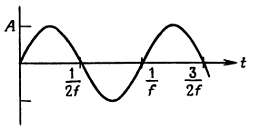
\includegraphics[width=0.575\textwidth]{../image/s_sin.png}
    \caption{Синусоидальный сигнал.}
	\end{figure}
Эффективное значение равняется двойной амплитуде, то есть размаху сигнала. 

Если нужно переместить начало координат ($t=0$) в какой-то момент времени, то в формулу следует добавить фазу:

$U=A sin2 \pi ft + \theta$

Синусоидальные сигналы характеризуются тремя параметрами:
\begin{itemize}
	\item $U_{M}$ или $I_{M}$ --- амплитуда переменного напряжения или тока;
	\item $f$ --- частота (период);
	\item $\theta$ --- фазовый сдвиг.
\end{itemize}

Данный тип сигналов является периодическим, т. е. временная зависимость повторяется и есть условия:

$u(t)=u(t+T)$

$ i(t)=i(t+T)$

где $T=\frac{1}{f}$ --- период повторения сигнала.

<<Основное достоинство синусоидальной функции (а также основная причина столь широкого распространения синусоидальных сигналов) состоит в том, что эта функция является решением целого ряда линейных дифференциальных уравнений, описывающих как физические явления, так и свойства линейных цепей.>>~\cite{is1}. Если подать на вход линейной цепи синусоидальный сигнал, то на выходе мы также получим синусоиду, но как правило с другой амплитудой и фазой. На практике поведение схемы оценивают по её амплитудно-частотной характеристике (АЧХ), которая показывает, как изменяется амплитуда синусоидального сигнала в зависимости от частоты. Для примера на усилителе звуковых частот амплитудно-частотная характеристика в идеале имеет ровную линию в диапазоне от 20 Гц до 20 кГц. Чаще всего частоты, с которыми приходится работать на синусоидальном сигнале, лежат в диапазоне от нескольких герц до нескольких мегагерц.

\subsection{Линейно-меняющийся сигнал}
Линейно-меняющийся сигнал --- это напряжение, возрастающее (или убывающее) с постоянной скоростью.

\begin{figure}[H]
     \begin{subfigure}[H]{0.45\textwidth}
         \centering
         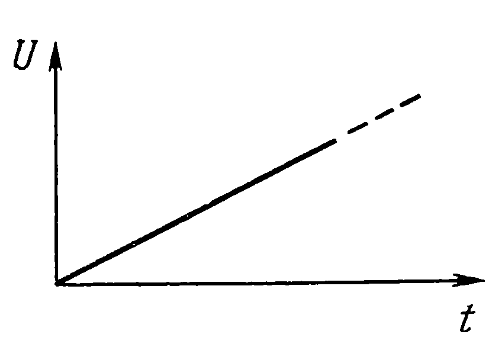
\includegraphics[width=0.70\textwidth]{../image/s_la.png}
         \caption{Возрастающее напряжение в виде сигнала.}
     \end{subfigure}
     \hfill
     \begin{subfigure}[H]{0.45\textwidth}
         \centering
         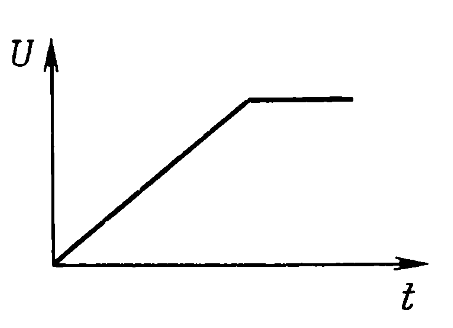
\includegraphics[width=0.70\textwidth]{../image/s_lb.png}
         \caption{Ограниченный сигнал.}
     \end{subfigure}
        \caption{Линейно-меняющийся сигнал.}
\end{figure}

Напряжение не может, конечно, расти бесконечно. Поэтому обычно данная величина имеет конечное значение (рис. 1.2 (б)) или сигнал становиться пилообразным (рис. 1.3).

	\begin{figure}[H]
    \centering
    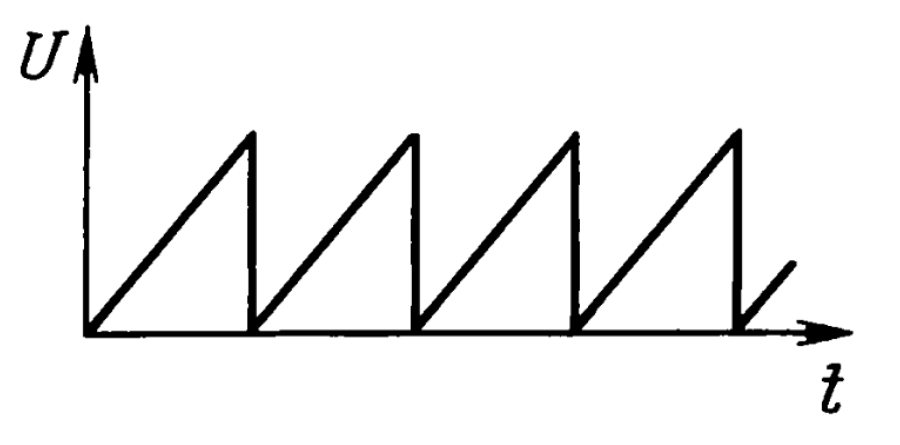
\includegraphics[width=0.5\textwidth]{../image/s_saw.png}
    \caption{Пилообразный сигнал.}
	\end{figure}

\subsection{Треугольный сигнал}
Треугольный сигнал очень похож на линейно-меняющийся, но его отличие в том, что он симметричный.

	\begin{figure}[H]
    \centering
    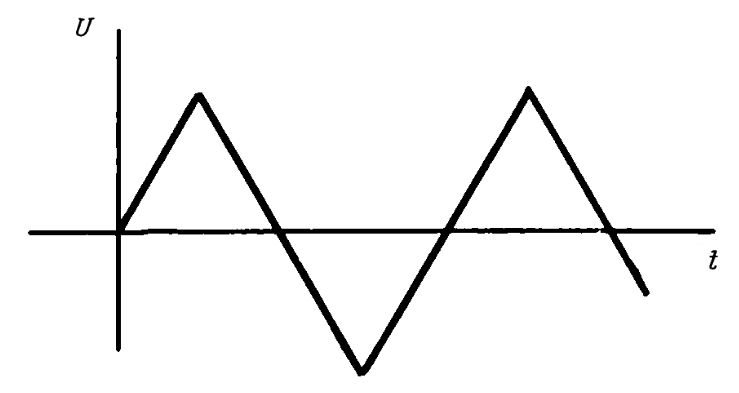
\includegraphics[width=0.5\textwidth]{../image/s_tri.png}
    \caption{Треугольный сигнал.}
	\end{figure}

%\subsection{Шум}

\subsection{Прямоугольный сигнал}
Прямоугольный сигнал или как его ещё называют меандр, характеризуется так же как и синусоидальный сигнал частотой и амплитудой.
	\begin{figure}[H]
    \centering
    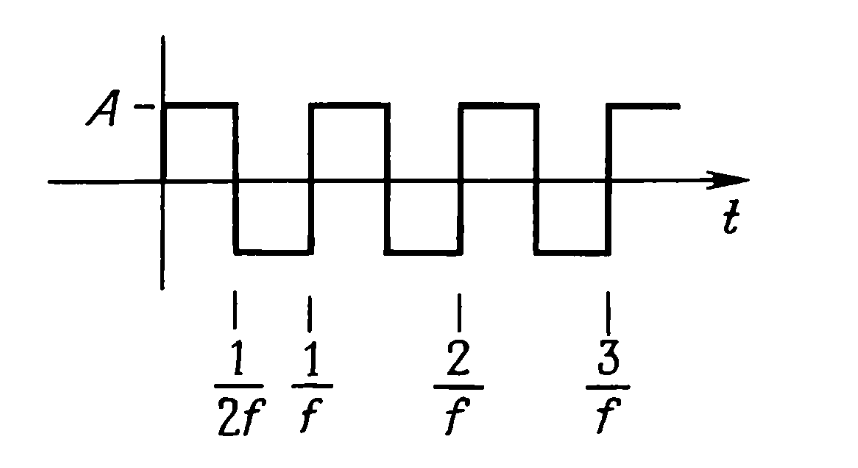
\includegraphics[width=0.55\textwidth]{../image/s_p.png}
    \caption{Прямоугольный сигнал.}
	\end{figure}

Если на вход линейной схемы подать прямоугольный сигнал, то на выходе вряд ли будет прямоугольник. Эффективным значением для данного сигнала является значение его амплитуды. <<Форма реального прямоугольного сигнала отличается от идеального прямоугольника; обычно в электронной схеме время нарастания сигнала $t_{H}$ составляет от нескольких наносекунд до нескольких микросекунд.>>~\cite{is1}. 

	\begin{figure}[H]
    \centering
    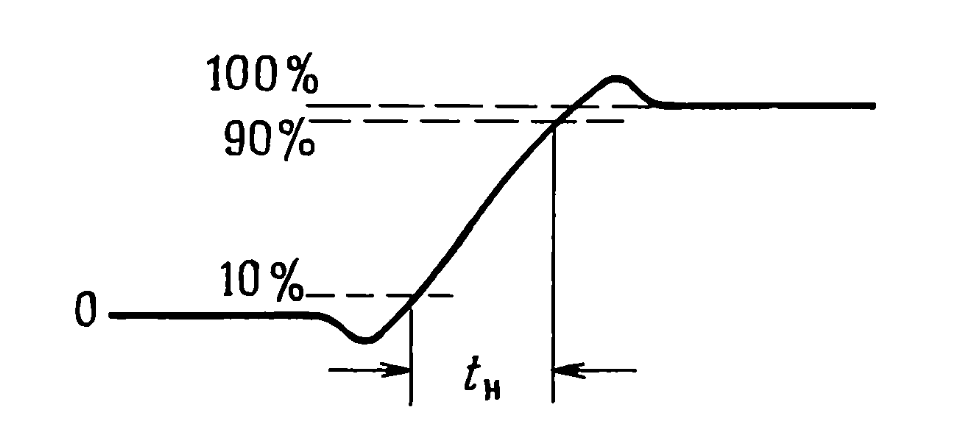
\includegraphics[width=0.65\textwidth]{../image/s_p_t.png}
    \caption{Время нарастания скачка прямоугольного сигнала.}
	\end{figure}
	
На рисунке 1.6 изображено как обычно выглядит скачок сигнала прямоугольника. Время когда сигнал нарастет определяется в промежутке от 10 до 90\% максимальной амплитуды сигнала.

\subsection{Импульсы}
Сигналы в виде импульса изображены на рисунке 1.7.

	\begin{figure}[H]
    \centering
    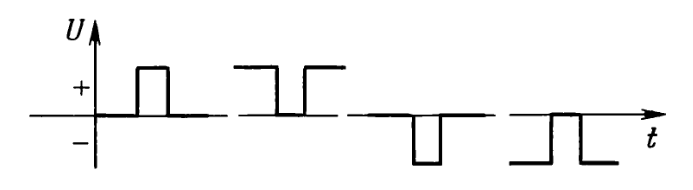
\includegraphics[width=0.65\textwidth]{../image/s_i.png}
    \caption{Прямоугольный сигнал.}
	\end{figure}
	
Данный вид сигналов характеризуется амплитудой и длительностью импульса. Можно генерировать последовательность периодических импульсов и тогда можно ещё характеризовать сигнал частотой (повторением импульса). У импульсов есть полярность --- положительная и отрицательная. Кроме этого импульс может спадать, а может нарастать. 
	


\subsection{Скачки и пики}
Часто можно слышать о сигналах в виде скачков и пиков, но на самом деле широкого применения они не находят. <<К их помощи прибегают для описания работы схем>>~\cite{is1}. Данный вид сигналов изображён на рисунке 1.8.

	\begin{figure}[H]
    \centering
    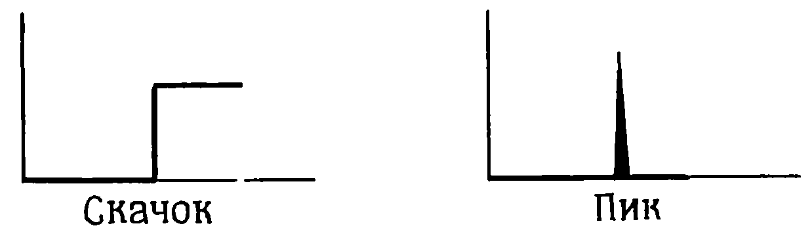
\includegraphics[width=0.55\textwidth]{../image/s_sp.png}
    \caption{Сигнал в виде скачка и пика.}
	\end{figure}

Скачок представляет из себя отдельную часть прямоугольного сигнала, в то время как пик представляет собой два скачка, разделенных очень коротким промежутком.


\section{Виды генераторов}
Источник сигнала часто является неотъемлемой частью схемы, но для тестирования работы удобно иметь отдельный, независимый источник сигнала. В качестве такого источника могут использоваться следующие виды генераторов.
\begin{enumerate}
	\item Генераторы синусоидальных сигналов.
	\item Функциональные генераторы.
	\item Генераторы сигналов произвольной формы.
	\item Генераторы импульсов.
\end{enumerate}

\subsection{Генераторы синусоидальных сигналов}
Генераторы таких сигналов широко применяются при тестировании различных радиоэлектронных устройств. <<Достоинством обычных генераторов синусоидальных сигналов является возможность получения синусоидальной формы выходного сигнала с малыми нелинейными искажениями. А главным недостатком — низкая стабильность частоты.>>~\cite{dgs}. Сами же синусоидальные сигналы являются простейшими. Они изменяются во времени, но их параметры --- амплитуда, частота и фаза остаются постоянными. Изменяя эти параметры, возможно осуществить модуляцию синусоидальных сигналов и использовать их для переноса информации. На таком принципе построены разнообразные области применения синусоидальных сигналов в технике электросвязи и радиотехнике.

В области измерительных приборов существуют различные виды генераторов синусоидального напряжения:

\begin{enumerate}
	\item Высокочастотные LC-генераторы.
	\item Низкочастотные RC-генераторы.
	\item Генераторы с разными типами резонаторов (кварцевые, пьезоэлектрические).
	\item Генераторы, которые формируют синусоиды, плавно ограничивая сигнал треугольника.
	\item Генераторы построенные на основе цифровых методах синтеза синусоидального сигнала.
\end{enumerate}

Конечно в настоящее время первые четыре типа генераторов уже прошлый век. Развитие цифровых и вычислительных технологий способствовало созданию и широкому распространению генераторов пятого типа, которые используют цифровые методы для генерации синусоидальных и различных других форм сигналов.

\subsection{Функциональные генераторы}
Функциональными генераторами обычно называют генераторы, которые могут создавать несколько функциональных зависимостей. Данные устройства генерируют сигналы разной формы. Их простота и плавная регулировка частоты в большом диапазоне привела к массовому применению генераторов такого типа. Из всех генераторов, генераторы функций являются очень гибкими. Они позволяют генерировать синусоидальные, треугольные и прямоугольные сигналы в широком спектре частот, при этом возможно регулировать амплитуду и смещать сигнал по постоянному току. Благодаря такому разнообразию сигналов, сфера применения таких генераторов сильно расширяется. Данный вид источника сигнала может быть одним на все случаи жизни. Их можно использовать для тестирования, исследования и отладки абсолютно разной электронной аппаратуры. <<Наиболее часто функциональные генераторы используются при отладке ВЧ, НЧ и сверхнизкочастотных устройств. В СВЧ диапазоне частот эти устройства не используются, за исключением применения в качестве источников модулирующих сигналов.>>~\cite{dgs}.

Функциональные генераторы также существуют как аналоговые так и цифровые, но в настоящее время аналоговые неактуальны. Переход к к функциональным генераторам с цифровым синтезов выходных сигналов и цифровой элементной базой связан с растущими требованиями к сигналам источника. У сигнала должна быть стабильная частота с амплитудой и верная форма. Благодаря применению цифровых элементов в массовой продукции (персональный компьютер, мобильный телефон), цифровые интегральные схемы стали бурно развиваться. Стала повышаться функциональность схем и понижаться их стоимость.



\subsection{Генераторы сигналов произвольной формы}
Данный вид генератора дополняет функциональный генератор. Достаточно новое направление в генераторах сигналов, которое основывается на прямом цифровом синтезе различных сигналов, по сути произвольных форм. Прямой цифровой синтез открыл возможность построить новую группу цифровых генераторов сигналов --- как обилие стандартных функций, так и произвольных форм. Однако синтез сигналов произвольных форм неминуемо усложняет устройство, <<так как требует применения перепрограммируемой электрическим способом памяти, введения редактора форм сигналов и средств отображения синтезируемой формы сигнала.>>~\cite{dgs}. Следовательно, генераторы такого типа относятся к достаточно сложным и дорогим приборам.

И всё же в ряде случаев данный вид генератора сигналов бывает очень необходим. С ростом сложности связной, телекоммуникационной, телевизионной и радиолокационной техники, увеличивается разнообразие форм сигналов, требующих тестирования.


\subsection{Генераторы импульсов}
Важно иногда передавать значительное количество энергии за короткий промежуток времени. Генерация импульсов необходима для тестирования и отладки импульсных систем. Это может быть радиолокатор или устройства и цифровые системы различного назначения. В радиолокации импульс направляется в пространство затем отражается от достигнутой цели и воспринимается радиолокационным приёмником. Получив информацию о времени задержки отражённого сигнала, можно оценить расстояние до цели, а проанализировав отражённый импульс можно сделать какие-то выводы о характере цели. Такого рода генераторы находят большое применение в качестве источников несинусоидальных сигналов. <<Импульсные сигналы нужны и в целом ряде других применений, например для запуска мощных лазерных диодов, построения ультразвуковых и видеоимпульсных локаторов, запуска ядерных и термоядерных процессов и даже при испытании многих электронных устройств, использующих импульсные сигналы или отдельные их свойств.>>~\cite{dgs}.


\section{Методы цифровой генерации сигнала}

	После рассмотрения видов генераторов сигналов можно сделать вывод о том, что способы получения сигнала также делятся на аналоговые и цифровые. Однако, в настоящее время аналоговые генераторы неактуальны и изучать способы генерации и схемы на аналоговой элементной базе большого смысла не имеет. Следует провести исследование цифровых методов генерации сигнала. 
	
	Метод аппроксимации подразумевает собой вычисление отсчётов функции по заданным параметрам. <<В памяти устройства хранятся лишь параметры генерируемого сигнала. Программа вычисляет отсчеты функции с некоторым заданным интервалом.>>~\cite{leso}. Исходя из этого, данный метод позволяет затратить небольшой объём памяти, но его недостаток это затраты на вычисления, что ограничивает максимальную частоту сигнала. 

	Для генерации сигналов также применяется итерационный метод CORDIC. <<CORDIC --- это аббревиатура от Coordinate Rotation Digital Computer: цифровое вычисление поворота системы координат. Алгоритм "цифра за цифрой" был разработан для аппаратного поворота вектора на плоскости с помощью простых операций "сдвиг регистра вправо" и сложение/вычитание регистров.>>~\cite{cordic}.
	
	
		
	В табличном методе генерации сигналов предполагается, что заранее вычисленные отсчёты хранятся в памяти. То есть никаких вычислений не требуется и генерация сводится к тому, что в порт цифро-аналогового преобразователя нужно вывести ячейку по заданному адресу. Таким образом, время на формирование отсчёта становится меньше и появляется возможность генерировать сигнал с более высокой частотой. Недостатком же является большие затраты памяти.
	

\section{Вывод из первой главы}
	
	
	